\chapter{Lecture 2 - Thermodynamic Analysis with EasyProp}
\label{ch:ch2}
\section{Objectives}
The objectives of this lecture are:
\begin{itemize}
\item Describe the EasyProp tools
\item Provide options for access to EasyProp
\item Do an Example Rankine cycle calculation with EasyProp
\end{itemize}

\section{The EasyProp Tools}

\begin{marginfigure}
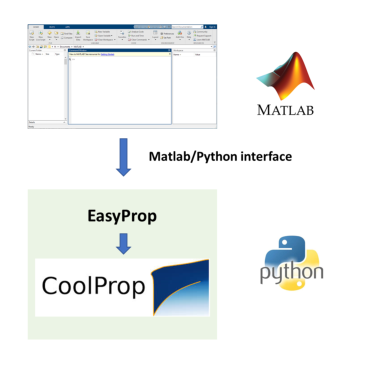
\includegraphics{Matlab-EasyProp-Schematic.pdf}
\caption{Schematic relationship between MATLAB and EasyProp}
\label{fig:matlab-easyprop}
\end{marginfigure}

What is EasyProp? \index{EasyProp}

\begin{itemize}
\item A library written in the Python language based on the free and open-source library CoolProp.  A schematic representation of the relationship between MATLAB, Python and the EasyProp and CoolProp Python libraries is given in Figure \ref{fig:matlab-easyprop}.
\item Accessible in a MATLAB environment with a properly initialized call to \emph{pyversion}\sidenote{The MATLAB function \emph{pyversion} sets several MATLAB environment variables that have the primary effect of ``telling'' MATLAB the path to the Python implementation that should be used when executing MATLAB scripts that use Python objects.}
\end{itemize}
How do I access EasyProp?

\begin{enumerate}
\item Login to \emph{ESSEX} via remote desktop and use any version of MATLAB installed
\begin{enumerate}
\item All software tools and libraries needed to use EasyProp have already been installed on this platform.
\item Users \emph{may} need to run \emph{pyversion\_fixer.m}\marginnote{The script \emph{pyversion\_fixer.m} will be made available to students as necessary.} to invoke the MATLAB built-in function \emph{pyversion} with the path to the local Python installation on \emph{ESSEX}.
\end{enumerate}
\end{enumerate}
Or
\begin{enumerate}[resume]
\item Install the required Python and MATLAB tools on your own laptop.
\begin{enumerate}
\item Download Anaconda (Anaconda3, Windows 64-bit, Python version 3.8) \marginnote[-2.25cm]{\textbf{Note: }If you opt for this method, you will have Python installed on your own laptop.  This is worthwhile.  When you graduate from USNA you will lose access to MATLAB along with many of the other non-free software packages that you may have become accustomed to using as a midshipman.  You can take Python with you and it can become the most powerful tool in your computational toolbox.}
\item From Anaconda prompt: conda install -c conda-forge coolprop
\item Locate Python executable.  One way to do this is from Anaconda prompt use the command: where python
\item In MATLAB call \emph{pyversion} with path to Python executable. E.g. >>pyversion('[path to python executable]')
\end{enumerate}
\end{enumerate}

\section{EasyProp Interface}
\newthought{A succinct introduction} to the EasyProp interface is available in the appendices.  For the remainder of this lecture I will try to exemplify the \emph{structure} of a MATLAB script in which EasyProp is being used.  I will follow this with a worked example where EasyProp is used to analyze a simple ideal Rankine Cycle.

\newthought{A basic analysis script} using EasyProp will flow as follows:

\begin{enumerate}
\item Ensure the Python system path includes the current directory 
\end{enumerate}


This is accomplished with the following code:\marginnote{Notice that we use the MATLAB commands 
\emph{clear}, \emph{clc}, and \emph{close 'all'}.  This is done in observation of the MATLAB Style requirement that we start every script with these three commands.  

MATLAB Style requirements are specified in the Appendix however I will use repetition in the lecture notes in an attempt to provide added emphasis.
}
\begin{lstlisting}[caption=Add the current directory to the Python system path, label={EP_setPath}]
%% Prepare the environment
clear;
clc;
close 'all';

EasyProp_path = ' '; %<- Path if EasyProp.py is in your current directory
if count(py.sys.path,EasyProp_path) == 0  % <-- see if desired directory is on path
    insert(py.sys.path,int32(0),EasyProp_path); %<-- if not; add it.
end
\end{lstlisting}

\begin{enumerate}[resume]
\item Construct a simple fluid object.
\end{enumerate}\marginnote{The leading \emph{py} tells MATLAB that what follows must be executed by the Python interpreter. The \emph{EasyProp} points to a particular Python library, and \emph{simpleFluid} is a function call within the EasyProp library.  The function \emph{simpleFluid} is a special type of function called a \emph{constructor}.}
\begin{lstlisting}[caption=Construct a \emph{simpleFluid} object]
units = 'USCS';
fluid = 'Water';
water = py.EasyProp.simpleFluid(fluid, units);
\end{lstlisting}
A list of common fluids that we will use in this course is provided in Table \ref{tab:fluid_list}.
\begin{margintable}
\begin{tabular}{cc}
\toprule
Fluid & EasyProp Name \\
\midrule
water & 'Water' \\
air & 'Air' \\
Carbon Dioxide & 'CO$_2$' \\
Nitrogen & 'N2' \\
Helium & 'He' \\
Refrigerant R245fa & 'R245fa' \\
\bottomrule
\end{tabular}
\caption{Commonly used EasyProp fluid designations}
\label{tab:fluid_list}
\end{margintable}

\begin{enumerate}[resume]
\item Establish problem parameters
\end{enumerate}

\begin{lstlisting}[caption=Set problem parameters]
numSp = 4; % number of state points
eta_turbine = 1.0; % isentropic efficiency of the turbine and pump
eta_pump  = 1.0;
Pmax = 838; % psia, max pressure
Pmin = 1.5; % psia, min pressure
\end{lstlisting}

\begin{enumerate}[resume]
\item Allocate fluid property arrays \marginnote{Pre-allocation of arrays is mandated in the ER468 style rules.  In this example we construct the arrays using the \emph{nan} function which, besides allocating memory for the arrays, initializes each value to ``Not-a-number'' (or \emph{nan}).  ``Not-a-number'' is preferred because it can never be mistaken for a number and thus can never be mistaken for a valid property value. This avoids the common logical error of using an array value with some incorrect-but-valid initial value (like zero).}  
\end{enumerate}

\begin{lstlisting}[caption=Allocate arrays to hold fluid property data.]
%% declare fluid property arrays
h = nan(numSp,1);
h_s = nan(numSp,1);
s = nan(numSp,1);
s_s = nan(numSp,1);
P = nan(numSp,1);
T = nan(numSp,1);
T_s = nan(numSp,1);
\end{lstlisting}

\begin{enumerate}[resume]
\item Determine fluid properties by using the functions associated with the EasyProp simpleFluid object.
\end{enumerate}

An example function call as follows: water.h\_pT(14.7,25)

\begin{equation*}
\underbracket{\text{water}}_{\text{object}}.\underbracket{\text{h\_pT}}_{\text{function}}\underbracket{\text{(14.7,25)}}_{\text{arguments}}
\end{equation*}

The "object" is the name of the Python object constructed in the step above.  The function name is given by convention;\marginnote[-3cm]{\textbf{Note: }Function name convention: [output property]\_[input property][input property](Arg 1, Arg 2).  In most cases the output thermodynamic property is determined based on two other known properties. In the case given, enthalpy (h) is determined as a function of pressure (p) and temperature (T)} in this case the property to be returned is the fluid enthalpy as a function of pressure and temperature.  The arguments - 14.7 and 25 - are the corresponding pressure and temperature; in this unit system they are given in units of psia and degrees Fahrenheit respectively.
\begin{margintable}
\begin{tabular}{lc}
\toprule
Property & EasyProp Abbreviation \\
\midrule
Pressure & p \\
Temperature & T \\
enthalpy & h \\
internal energy  & u \\
entropy & s \\
specific volume  & v \\
quality & x \\
viscosity & mu \\
\bottomrule
\end{tabular}
\caption{Property abbreviations}
\label{tab:property-list}
\vspace{0.5cm}
\end{margintable}

A list of fluid property abbreviations is given in Table \ref{tab:property-list}.  A list of units for each property used in the SI and USCS unit systems is given in Table \ref{tab:unit-list}.


\begin{margintable}
\begin{tabular}{lcc}
\toprule
Property & SI & USCS \\
\midrule
Temperature & C & F \\
Pressure & kPa & psia \\
enthalpy & kJ/kg & BTU/lbm \\
\bottomrule
\end{tabular}
\caption{EasyProp units}
\label{tab:unit-list}
\end{margintable}

\newthought{The remaining functions} needed to determine fluid properties at the state points are given in the listing below.

\begin{lstlisting}[caption=Find fluid properties for each state point in a simple Rankine cycle.]
%% calculate properties at state points 
% state point 1 - condenser outlet condensate pump inlet
P(1) = Pmin;
h(1) = myFluid.hL_p(P(1));
s(1) = myFluid.sL_p(P(1));

% compression from state point 1 to state point 2
P(2) = Pmax;
s_s(2) = s(1);
h_s(2) = myFluid.h_ps(P(2),s_s(2));
h(2) = h(1) - (h(1) - h_s(2))./eta_pump;

w_pump = h(1) - h(2);

% isobaric heat addition in the boiler from state point 2 to state point 3
P(3) = P(2);
h(3) = myFluid.hV_p(P(3));
s(3) = myFluid.sV_p(P(3));

q_s = h(3) - h(2);

% expansion in turbine from state point 3 to state point 4
P(4) = P(1);
s_s(4) = s(3);
h_s(4) = myFluid.h_ps(P(4),s_s(4));
h(4) = h(3) - eta_turbine*(h(3) - h_s(4));

w_turbine = h(3) - h(4);

% isobaric heat rejection in the condenser from sp 4 to sp 1
q_r = h(1) - h(4);
\end{lstlisting}

\begin{enumerate}[resume]
\item Complete analysis to find thermal efficiency and net work
\end{enumerate}
\begin{lstlisting}[caption=Analyze for net work and thermal efficiency]
%% First Law Check
w_net = w_pump + w_turbine;
q_net = q_s + q_r;

fprintf('Net work = %g kJ/kg \n',w_net);
fprintf('Net heat = %g kJ/kg \n',q_net);

%% Compute Thermal Efficiency
eta_th = w_net/q_s;

fprintf('Thermal efficieency = %4.1f percent \n',eta_th*100);
\end{lstlisting}

\newthought{There is more to analyze} than simply obtaining values for net specific work and thermal efficiency. Some fundamental things to think about:
\begin{enumerate}
\item Are my results correct?  In general it is difficult to know; most relevant problems do not come with a solution key.  You should take steps to increase your confidence that your answer is sensible.  A few essential steps include:
\begin{enumerate}
\item If you have computed net specific work, you should also compute net specific heat ($q_{net}$) and verify that they are, to within reasonable limits of precision, equal to each other. \sidenote[][-1cm]{When using a tool like EasyProp, $q_{net}$ and $w_{net}$ should be well within 1 BTU/lb$_{\text{m}}$ or 1 kJ/kg of each other.  If not, you probably have a bug somewhere.}
\item Is your computed thermal efficiency less than the Carnot efficiency?  If not: it is definitely wrong.
\item How does this answer compare to your results for a similar cycle?  Do the differences make sense? or
\item If you make small changes to the problem parameters---e.g. you slightly change the maximum/minimum system temperature/pressure---does that result in the expected change to net work and thermal efficiency?
\end{enumerate}
\item What are the strengths and weaknesses of the cycle that I have just analyzed? What could I change to make it better?  
\end{enumerate}
Answers to the question above cannot be given in general but you will become better at answering them with practice.  This course is designed to give you plenty of practice.



